\documentclass[a4paper,11.5pt]{article}
\usepackage[textwidth=170mm, textheight=230mm, inner=20mm, top=20mm, bottom=30mm]{geometry}
\usepackage[normalem]{ulem}
\usepackage[utf8]{inputenc}
\usepackage[T1]{fontenc}
\PassOptionsToPackage{defaults=hu-min}{magyar.ldf}
\usepackage[magyar]{babel}
\usepackage{amsmath, xcolor, amsthm,amssymb,paralist,array, ellipsis, graphicx, tikz}
\usetikzlibrary{shapes.geometric, arrows, positioning}
%\usepackage{marvosym}

\usepackage{listings}
\lstset{
	language=C++, 
	basicstyle=\ttfamily, 
	keywordstyle=\color{blue}\ttfamily, 
	stringstyle=\color{red}\ttfamily,
	tabsize = 4
}

\makeatletter
\renewcommand*{\mathellipsis}{%
	\mathinner{%
		\kern\ellipsisbeforegap%
		{\ldotp}\kern\ellipsisgap%
		{\ldotp}\kern\ellipsisgap%
		{\ldotp}\kern\ellipsisaftergap%
	}%
}
\renewcommand*{\dotsb@}{%
	\mathinner{%
		\kern\ellipsisbeforegap%
		{\cdotp}\kern\ellipsisgap%
		{\cdotp}\kern\ellipsisgap%
		{\cdotp}\kern\ellipsisaftergap%
	}%
}
\renewcommand*{\@cdots}{%
	\mathinner{%
		\kern\ellipsisbeforegap%
		{\cdotp}\kern\ellipsisgap%
		{\cdotp}\kern\ellipsisgap%
		{\cdotp}\kern\ellipsisaftergap%
	}%
}
\renewcommand*{\ellipsis@default}{%
	\ellipsis@before
	\kern\ellipsisbeforegap
	.\kern\ellipsisgap
	.\kern\ellipsisgap
	.\kern\ellipsisgap
	\ellipsis@after\relax}
\renewcommand*{\ellipsis@centered}{%
	\ellipsis@before
	\kern\ellipsisbeforegap
	.\kern\ellipsisgap
	.\kern\ellipsisgap
	.\kern\ellipsisaftergap
	\ellipsis@after\relax}
\AtBeginDocument{%
	\DeclareRobustCommand*{\dots}{%
		\ifmmode\@xp\mdots@\else\@xp\textellipsis\fi}}
\def\ellipsisgap{.1em}
\def\ellipsisbeforegap{.05em}
\def\ellipsisaftergap{.05em}
\makeatother

\usepackage{hyperref}

\begin{document}
	%%%%%%%%%%%RÖVIDÍTÉSEK%%%%%%%%%%
	\setlength\parindent{0pt}
	\def\s{\hspace{0.2mm}\vphantom{\beta}}
	\def\Z{\mathbb{Z}}
	\def\Q{\mathbb{Q}}
	\def\R{\mathbb{R}}
	\def\C{\mathbb{C}}
	\def\N{\mathbb{N}}
	\def\Ra{\overline{\mathbb{R}}}
	
	\def\sume{\displaystyle\sum_{n=1}^{+\infty}}
	\def\sumn{\displaystyle\sum_{n=0}^{+\infty}}
	
	\def\narrow{\underset{n\rightarrow+\infty}{\longrightarrow}}
	\def\limn{\displaystyle\lim_{n\to +\infty}}
	\def\limx{\displaystyle\lim_{x\to +\infty}}
	
	\theoremstyle{definition}
	\newtheorem{theorem}{Tétel}[subsection] 
	
	\theoremstyle{definition}
	\newtheorem{definition}[theorem]{Definíció} 
	\newtheorem{example}[theorem]{Példa} 
	\newtheorem{task}[theorem]{Feladat} 
	\newtheorem{note}[theorem]{Megjegyzés}
	%%%%%%%%%%%%%%%%%%%%%%%%%%%%%%%%%%%%%%%%%%%%%%%%%%%%%%%%%%%%%%%%%%%%%
	\begin{center}
		{\LARGE\textbf{C++}}
		
		{\Large Gyakorlat jegyzet}
		
		2 óra.
	\end{center}
	A jegyzetet \textsc{Umann} Kristóf készítette \textsc{Porkoláb} Zoltán és \textsc{Horváth} Gábor. (\today)
	
	%TODO függvény és operátor túlterhelés ide illene a legjobban
	%TODO globális és statikus függvényeket is ide kéne beilleszteni
	
	
	\section{Láthatóság, élettartam}
	Egy objektum \textbf{láthatóságának} nevezzük a kódnak azon szakaszait, melyeknél lehet rá hivatkozni.
	\smallskip
	
	Egy objektum \textbf{élettartamának} nevezzük a kód azon szakaszát, melynél bent szerepel a memóriában. Amikor egy objektum élettartama elkezdődik, azt mondjuk, az objektum létrejön, míg az élettartam végén az objektum megsemmisül.
	\medskip
	\begin{note}
		Ez alapján megállapíthatjuk, hogy egy globális változó láthatósága és élettartama a program futásának elejétől végéig tart.
	\end{note}
	
	Figyeljük meg, mikor tudunk \texttt{x} változóra hivatkozni (azaz hol lesz \texttt{x} látható)!
	\begin{lstlisting}
int x;

int main()
{
	int x = 1;
	{
		int x = 2;
		std::cout << x << std::endl; // 2
	}
}
	\end{lstlisting}
	Megfigyelhető, hogy a \texttt{main} függvény elején létrehozott \texttt{x} az utána következő blokkban teljesen elérhetetlen -- nincs olyan szabványos nyelvi eszköz, amivel tudnánk rá hivatkozni. Ezt a folyamatot \textbf{leárnyékolás}nak (\textit{shadowing}) nevezzük. Azonban a külső, globális \texttt{x}-re bármikor tudunk hivatkozni az alábbi módon:
	\begin{lstlisting}
int x;

int main()
{
	int x = 1;
	{
		int x = 2;
		std::cout << ::x << std::endl; // 0
	}
}
	\end{lstlisting}
	
	\section{A stack működése}
	A stack a c++ alapértelmezett ,,memóriája'', minden változó alapértelmezetten itt jön létre és semmisül meg. Amennyiben egy változóra többet nem tudunk hivatkozni, automatikusan megsemmisül.
	
	\begin{lstlisting}
#include <iostream>

int f()
{
	int x = 0; //x letrejon
	++x;
	return x;
} //x megsemmisul

int main()
{
	std::cout << f() << std::endl;
	std::cout << f() << std::endl;
	std::cout << f() << std::endl;
	std::cout << f() << std::endl;
	std::cout << f() << std::endl;
}
	\end{lstlisting}
	Kimenet: \texttt{1 1 1 1 1}
	\medskip
	
	A fenti kód működését így képzelhetjük el:
	
	%durva kód copy paste inc... dont be mad :'(
	\begin{center}
		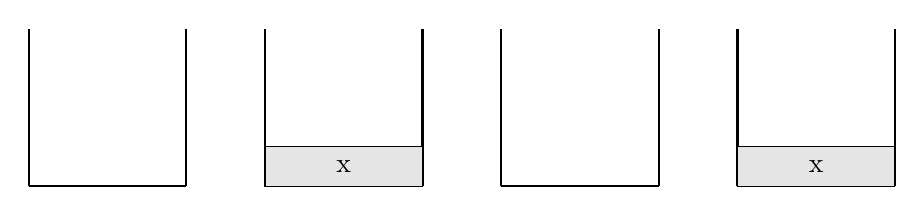
\begin{tikzpicture}
		\tikzstyle{Node} = [rectangle, minimum width=2cm, minimum height=5mm, text centered, draw=black, fill= gray!20]
		\tikzstyle{arrow} = [thick,->,>=stealth]
		
		
		\draw [thick, black] (-3, 0) -- (-1, 0);
		\draw [thick, black] (-3, 0) -- (-3, 2);
		\draw [thick, black] (-1, 0) -- (-1, 2);
		
		\draw [thick, black] (0, 0) -- (2, 0);
		\draw [thick, black] (0, 0) -- (0, 2);
		\draw [thick, black] (2, 0) -- (2, 2);
		\node (x) [Node] at (1,0.25) {x};
		
		\draw [thick, black] (3, 0) -- (5, 0);
		\draw [thick, black] (3, 0) -- (3, 2);
		\draw [thick, black] (5, 0) -- (5, 2);
		
		\draw [thick, black] (6, 0) -- (8, 0);
		\draw [thick, black] (6, 0) -- (6, 2);
		\draw [thick, black] (8, 0) -- (8, 2);
		\node (x) [Node] at (7,0.25) {x};
		\end{tikzpicture}
	\end{center}
	Az ábrán egy stack-et látunk. Amikor a vezérlés az \texttt{f} függvényhez ér, és ott létrehozza az \texttt{x} változót, azt behelyezi a stack-be. A \texttt{return} kulcsszó hatására készít \texttt{x}-ről egy temporális példányt, ami a függvény visszatérési értéke lesz. Amikor a vezérlés visszatér a \texttt{main} függvényhez, {x}-re nem tudunk tovább hivatkozni, így azt megsemmisíti, és ez ismétlődik folyamatosan.
	\smallskip
	
	A stack egy FILO (\textit{first in last out}) adatszerkezet -- azaz azt az elemet ,,dobja'' ki a vezérlés a stack-ből, melyet utoljára rakott be.
	
	\section{Paraméter átvétel}
	\subsection{Érték szerinti paraméter átvétel}
	Próbáljuk megvalósítani a swap függvényt!
	%http://tex.stackexchange.com/questions/228724/how-do-i-make-tikz-make-a-curved-arrow-from-one-node-to-another-when-my-nodes-ar
	\begin{lstlisting}
#include <iostream>
void swapWrong(int a, int b)
{
	int tmp = a;
	a = b;
	b = a;
}

int main()
{
	int c = 5, d = 8;
	swap(c, d);
	std::cout << c << ' ' << d << std::endl;
}
	\end{lstlisting}		
	A program kimenete \texttt{5 8} ment. Ez egy teljesen jól definiált viselkedés. Ez azért van, mert itt \textbf{érték} szerint vettük át (\textit{pass by value}) \texttt{a} és \texttt{b} változót. A következő ábrán megfigyelhetjük miért is nem. Képzeljük el, ahogy ebbe a verembe a kódunk elrakja a \texttt{c} és \texttt{d} változókat. Majd meghívja a \texttt{swapWrong} függvényt, melyben létrehozott \texttt{a} és \texttt{b} változókat ismét behelyezi. Bár a függvényre lokális \texttt{a} és \texttt{b} változókat megcseréli, de a függvényhívás után ezeket ki is törli a stackből.
	\begin{center}
		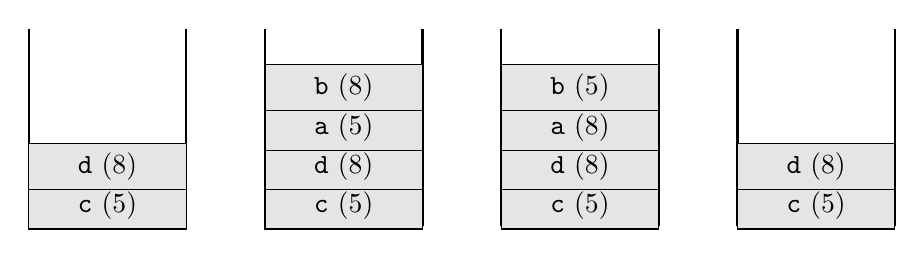
\begin{tikzpicture}
		\tikzstyle{Node} = [rectangle, minimum width=2cm, minimum height=5mm, text centered, draw=black, fill= gray!20]
		\tikzstyle{arrow} = [thick,->,>=stealth]
		
		\draw [thick, black] (-3, 0) -- (-1, 0);
		\draw [thick, black] (-3, 0) -- (-3, 2.5);
		\draw [thick, black] (-1, 0) -- (-1, 2.5);
		\node (c1) [Node] at (-2,0.25) {\texttt{c} (5)};
		\node (d1) [Node] at (-2,0.75) {\texttt{d} (8)};
		
		\draw [thick, black] (0, 0) -- (2, 0);
		\draw [thick, black] (0, 0) -- (0, 2.5);
		\draw [thick, black] (2, 0) -- (2, 2.5);
		\node (c2) [Node] at (1,0.25) {\texttt{c} (5)};
		\node (d2) [Node] at (1,0.75) {\texttt{d} (8)};
		\node (a2) [Node] at (1,1.25) {\texttt{a} (5)};
		\node (b2) [Node] at (1,1.75) {\texttt{b} (8)};
		
		\draw [thick, black] (3, 0) -- (5, 0);
		\draw [thick, black] (3, 0) -- (3, 2.5);
		\draw [thick, black] (5, 0) -- (5, 2.5);
		\node (c3) [Node] at (4,0.25) {\texttt{c} (5)};
		\node (d3) [Node] at (4,0.75) {\texttt{d} (8)};
		\node (a3) [Node] at (4,1.25) {\texttt{a} (8)};
		\node (b3) [Node] at (4,1.75) {\texttt{b} (5)};
		
		\draw [thick, black] (6, 0) -- (8, 0);
		\draw [thick, black] (6, 0) -- (6, 2.5);
		\draw [thick, black] (8, 0) -- (8, 2.5);
		\node (a4) [Node] at (7,0.25) {\texttt{c} (5)};
		\node (b4) [Node] at (7,0.75) {\texttt{d} (8)};
		\end{tikzpicture}
	\end{center}
	C++ban alapértelmezett a paraméterátadás függvényeknél érték szerint történik.
	\subsection{Mutatóval történő paraméter átvétel}
	A mutatók olyan nyelvi elemek, melyek egy memóriaterületre mutatnak. Segítségükkel anélkül is tudunk hivatkozni egy adott objektumra (és nem csak a másolatára), hogy közvetlenül az objektummal dolgoznánk. Most röviden megismerkedünk velük, de később részletesebben visszatérünk rájuk.
	\begin{lstlisting}
int main()
{
	int c = 5, d = 8;
	int *p = &c;
}
	\end{lstlisting}
	A fenti példában \texttt{p} egy mutató (\textit{pointer}), mely egy \texttt{int} típusra mutat. Ahhoz, hogy értéket tudjunk adni egy mutatónak, egy memóriacímet (\textit{referenciát}) kell neki értékül adni, amire rá tud mutatni, erre való a \textbf{referáló operátor} (\&). Ha a mutató által \textit{mutatott értéket} szeretnénk módosítani, akkor dereferálnunk kell a \textbf{dereferáló operátor}ral (*).
	\begin{lstlisting}
int *p = &c; //referaljuk c-t
*p = 4; //dereferaljuk p-t
p = &d;
*p = 7;
	\end{lstlisting}
	Rendre: pointer inicializálása, pointer által mutatott érték módosítása, pointer átállítása másik memóriacímre, és a mutatott érték módosítása.
	
	Egy mutató mutathat változóra, másik mutatóra, saját magára, és sehova is. Azok a mutatókak, melyek sehová sem mutatnak, nullpointernek nevezzük, és így hozhatjuk létre őket:
	
	{\centering \texttt{p = 0;\quad \quad p = NULL;\quad \quad p = nullptr;} \par}
	
	\begin{note}
		Ez a három értékadás (közel) ekvivalens, azonban a \texttt{nullptr} kulcsszó csak c++11ben érhető el.
	\end{note}
	
	\begin{lstlisting}
void swapP(int *a, int *b)
{
	int tmp = *a;
	*a = *b;
	*b = tmp;
}
	\end{lstlisting}
	
	Amennyiben ezt a függvényt hívjuk meg, valóban megcserélődik a két változó értéke. De ehhez fontos, hogy ne simán \texttt{swapP(c, d)}-t írjunk függvényhívásként, az ugyanis az fordítási hibához vezetne, mert a \texttt{c} és \texttt{d} típusa \texttt{int}, és nem \texttt{int*}. Ahhoz, hogy értéket adjunk egy pointernek, a \texttt{c}-hez és \texttt{d}-hez tartozó memóriacímeket kell átadni, így a \texttt{swapP(\&c, \&d)} hívás lesz megfelelő.
	\begin{center}
		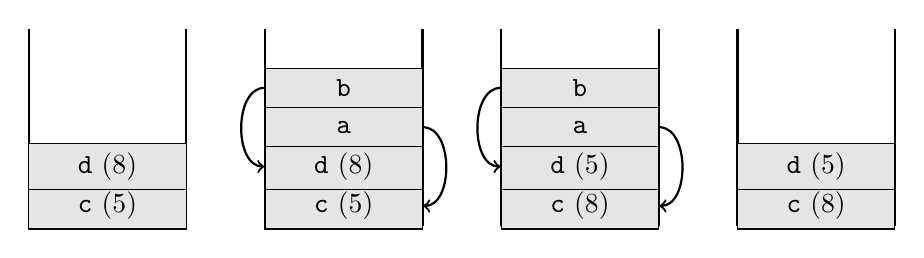
\begin{tikzpicture}
		\tikzstyle{Node} = [rectangle, minimum width=2cm, minimum height=5mm, text centered, draw=black, fill= gray!20]
		\tikzstyle{arrow} = [thick,->,>=stealth]
		
		\draw [thick, black] (-3, 0) -- (-1, 0);
		\draw [thick, black] (-3, 0) -- (-3, 2.5);
		\draw [thick, black] (-1, 0) -- (-1, 2.5);
		\node (c1) [Node] at (-2,0.25) {\texttt{c} (5)};
		\node (d1) [Node] at (-2,0.75) {\texttt{d} (8)};
		
		\draw [thick, black] (0, 0) -- (2, 0);
		\draw [thick, black] (0, 0) -- (0, 2.5);
		\draw [thick, black] (2, 0) -- (2, 2.5);
		\node (c2) [Node] at (1,0.25) {\texttt{c} (5)};
		\node (d2) [Node] at (1,0.75) {\texttt{d} (8)};
		\node (a2) [Node] at (1,1.25) {\texttt{a}};
		\node (b2) [Node] at (1,1.75) {\texttt{b}};
		
		\path[every node/.style={font=\sffamily\small}]
			(a2) edge[bend left = 90, thick, ->] node [right] {} (c2);
		\path[every node/.style={font=\sffamily\small}]
			(b2) edge[bend right = 90, thick, ->] node [left] {} (d2);
		
		\draw [thick, black] (3, 0) -- (5, 0);
		\draw [thick, black] (3, 0) -- (3, 2.5);
		\draw [thick, black] (5, 0) -- (5, 2.5);
		\node (c3) [Node] at (4,0.25) {\texttt{c} (8)};
		\node (d3) [Node] at (4,0.75) {\texttt{d} (5)};
		\node (a3) [Node] at (4,1.25) {\texttt{a}};
		\node (b3) [Node] at (4,1.75) {\texttt{b}};
		
		
		\path[every node/.style={font=\sffamily\small}]
		(a3) edge[bend left = 90, thick, ->] node [right] {} (c3);
		\path[every node/.style={font=\sffamily\small}]
		(b3) edge[bend right = 90, thick, ->] node [left] {} (d3);
		
		\draw [thick, black] (6, 0) -- (8, 0);
		\draw [thick, black] (6, 0) -- (6, 2.5);
		\draw [thick, black] (8, 0) -- (8, 2.5);
		\node (a4) [Node] at (7,0.25) {\texttt{c} (8)};
		\node (b4) [Node] at (7,0.75) {\texttt{d} (5)};
		\end{tikzpicture}
	\end{center}
	
	Ezt azonban ez még mindig \textbf{érték szerinti} átadásnak nevezzük, mert most nem konkrét értéket, hanem a memóriacímet másoltuk át.
	
	\begin{lstlisting}
void swapWrong2(int *a, int *b)
{
	int *tmp = a;
	a = b;
	b = tmp;
}
	\end{lstlisting}
	Ebben a példában nem a pointerek által mutatott értéket, hanem magukat a pointereket cseréljük meg. Itt annyi fog csupán történni, hogy a függvény beljesében \texttt{a} és \texttt{b} pointer másra fog mutatni. De annak értéke nem változik.
	
	\begin{center}
		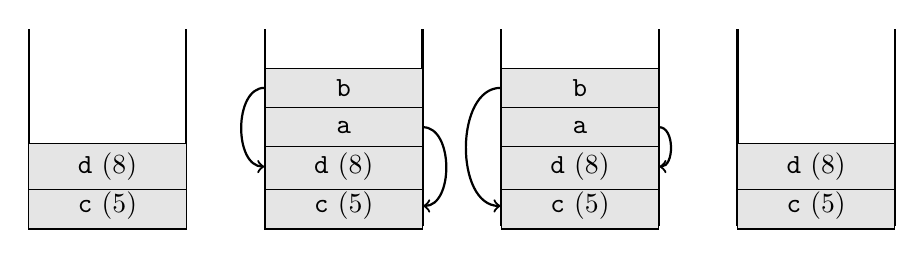
\begin{tikzpicture}
		\tikzstyle{Node} = [rectangle, minimum width=2cm, minimum height=5mm, text centered, draw=black, fill= gray!20]
		\tikzstyle{arrow} = [thick,->,>=stealth]
		
		\draw [thick, black] (-3, 0) -- (-1, 0);
		\draw [thick, black] (-3, 0) -- (-3, 2.5);
		\draw [thick, black] (-1, 0) -- (-1, 2.5);
		\node (c1) [Node] at (-2,0.25) {\texttt{c} (5)};
		\node (d1) [Node] at (-2,0.75) {\texttt{d} (8)};
		
		\draw [thick, black] (0, 0) -- (2, 0);
		\draw [thick, black] (0, 0) -- (0, 2.5);
		\draw [thick, black] (2, 0) -- (2, 2.5);
		\node (c2) [Node] at (1,0.25) {\texttt{c} (5)};
		\node (d2) [Node] at (1,0.75) {\texttt{d} (8)};
		\node (a2) [Node] at (1,1.25) {\texttt{a}};
		\node (b2) [Node] at (1,1.75) {\texttt{b}};
		
		\path[every node/.style={font=\sffamily\small}]
		(a2) edge[bend left = 90, thick, ->] node [right] {} (c2);
		\path[every node/.style={font=\sffamily\small}]
		(b2) edge[bend right = 90, thick, ->] node [left] {} (d2);
		
		\draw [thick, black] (3, 0) -- (5, 0);
		\draw [thick, black] (3, 0) -- (3, 2.5);
		\draw [thick, black] (5, 0) -- (5, 2.5);
		\node (c3) [Node] at (4,0.25) {\texttt{c} (5)};
		\node (d3) [Node] at (4,0.75) {\texttt{d} (8)};
		\node (a3) [Node] at (4,1.25) {\texttt{a}};
		\node (b3) [Node] at (4,1.75) {\texttt{b}};
		
		
		\path[every node/.style={font=\sffamily\small}]
		(a3) edge[bend left = 90, thick, ->] node [right] {} (d3);
		\path[every node/.style={font=\sffamily\small}]
		(b3) edge[bend right = 90, thick, ->] node [left] {} (c3);
		
		\draw [thick, black] (6, 0) -- (8, 0);
		\draw [thick, black] (6, 0) -- (6, 2.5);
		\draw [thick, black] (8, 0) -- (8, 2.5);
		\node (a4) [Node] at (7,0.25) {\texttt{c} (5)};
		\node (b4) [Node] at (7,0.75) {\texttt{d} (8)};
		\end{tikzpicture}
	\end{center}
	\subsection{Referencia szerinti paraméter átvétel}
	Megállapíthatjuk, hogy az előző megoldásnál nem változtattuk meg azt, hogy mire mutassanak a pointerek, így azokat konstansként is definiálhatnánk. A konstans pointerek módosíthatják a mutatott cím értékét, de máshova nem mutathatnak. Úgy tudunk egy ilyen pointert létrehozni, hogy a csillag után írjuk a \texttt{const} kulcsszót.
	\begin{lstlisting}
void swap(int * const a, int * const b)
{
	//...
}
	\end{lstlisting}
	Egy kis szintaktikai cukorkával megúszhatjuk azt, hogy folyton kiírjuk a \texttt{* const}-ot (lévén ritkán akarjuk megváltoztatni hogy ilyen esetben a pointer hova mutasson). Erre való a {referencia szerinti paraméter átváétel} (\textit{pass by reference}). A referencia úgy működik, mintha egy konstans pointer lenne.
	\begin{lstlisting}
void swapRef(int &a, int &b)
{
	int tmp = a;
	a = b;
	b = tmp;
}
	\end{lstlisting} 
	Ez a két függvény lényegében ekvivalensek. A különbség a referencia és a pointer között csupán annyi, hogy egy referencia nem lehet null.
	\begin{note}
		Ez bár ezt referencia szerinti átvételnek nevezzük, de itt is történik másolás, a memóriacímet ítt is érték szerint vesszük át.
	\end{note}
		Megjegyzendő, hogy a fenti \texttt{swapRef} függvénynek nem kell memóriacímeket átadni, \texttt{swapRef(a,b)}-t kell írnunk.
	\begin{note}
		Egy referenciát mindig inicializálni kell. Csak úgy mint egy konstanst (különben fordítási hibát kapunk.)
	\end{note}
	\section{Visszatérési érték problémája}
	Nem primitív (pl. \texttt{int}) típusoknál gyakran megeshet, hogy egy adott ípushoz tartozó pointer mérete kisebb, mint magának az objektumé, így megérheti mindentől függetlenül a paramétert referencia szerint átvenni. Ezen felbátorodva mondhatnánk azt is, hogy referenciával is térjünk vissza (a követekező példában tekintsünk el attól, hogy \texttt{int}-el dolgozunk, bátran képzeljük azt hogy az pl. egy nagyon nagy mátrix)!
	\begin{lstlisting}
int& addOne(int &i)
{
	i++;
	return i;
}

int main()
{
	int i = 0;
	int a = addOne(i);
	std::cout << a << std::endl;
}
	\end{lstlisting}
	A fenti kóddal semmi gond nincs is. De mi van, ha egy picit módosítunk rajta?
	\begin{lstlisting}
int& addOne(int &i)
{
	int ret = ++i;
	return ret;
}
	\end{lstlisting}
	A baj máris megvan, amit egy warning is jelezni fog nekünk: olyan objektumra hivatkozó referenciát adunk vissza, amely \texttt{addOne}-on belül lokális. Ez azt jelenti, hogy amint a vezérlés visszatér a \texttt{main} függvényhez, \texttt{ret} megsemmisül, és a \texttt{main} függvény pedig a \texttt{ret}-hez tartozó címen lévő értéket próbálná meg lemásolni. Mivel viszont a \texttt{ret} már ezen a ponton megsemmisült, semmi nem garantálja, hogy azon a memóriaterületen ne követekezett volna be módosítás.
	
	\medskip
	Az olyan memóriaterületre való hivatkozás, mely nincs a program számára lefoglalva, nem definiált viselkedést eredményez.
	\medskip
	
	\section{Kifejezések kiértékelése.}
	\begin{example}\ 
		
		\begin{lstlisting}
#include <iostream>

char* answer (char *q);

int main()
{
	std::cout << answer("Hogy vagy?") << answer("Biztos?") << std::endl;
	return 0;
}

char* answer (char *q)
{
	std::cout << q;
	static char buffer[80];
	std::cin.getline(buffer,80);
	return buffer;
}
		\end{lstlisting}
		Itt már azt is meg akarjuk kérdezni, hogy biztos-e. Itt már találkoztunk a problémával, hogy a kiíratás sorrendje rossz. 
		
		\texttt{std::cout $<<$ answer("Biztos?") $<<$ answer("Hogy vagy?") $<<$ std::endl;}
		
		Ez már jó. (a kiértékelés nem definiált, de a kiíratási sorrend igen!)
		
		Ez az igazán jó megoldás, itt kevesebbet kell filózni:
		
		\text{std::cout $<<$ answer("Hogy vagy?");}
		
		\texttt{std::cout $<<$ answer("Biztos?");}
		
	\end{example}
	
	Azonban a statikus változótól még nem szabadultunk meg. Egy másik megoldás lehet a dinamikus memória kezelés.
	\medskip
	
	A dinamikusan lefoglalt memória az ,,átlagos'' stacken lévő objektumokkal szemben a mi felelőségünk teljesen. Nekünk kell őket allokálni, és ha nincs már rá szükségünk, nekünk is kell felszabadítani. c++11ben smart-pointerekkel ezt valamelyest automatizálhatjuk.
		
		\begin{lstlisting}
#include <iostream>

char* answer (char *q);

int main()
{
	std::cout << answer("Hogy vagy?");
	std::cout << answer("Biztos?");
	return 0;
}

char* answer (char *q)
{
	std::cout << q;
	char* buffer = new char[80];
	std::cin.getline(buffer,80);
	return buffer;
}
		\end{lstlisting}
		Ez így nagyon szép megoldás, de a memória sajnos elúszott. Ahogy említve volt, a \texttt{new} kulcsszóval létrehoztunk a dinamikus tárhelyen egy új változót, de azt soha nem szabadítottuk fel. Ezért a legszebb megoldás még mindig az, hogyha referenciával átadok még egy paramétert, amiben el tudjuk tárolni a választ. Ennél azonban még egyszerűbb megoldás az, ha az \texttt{std::string}-et használjuk.
		\begin{lstlisting}
#include <iostream>

std::string answer (char *q);

int main()
{
	std::cout << answer("Hogy vagy?");
	std::cout << answer("Biztos?");
	return 0;
}

std::string answer (std::string q)
{
	std::cout << q;
	std::string buffer;
	std::cin >> buffer;
	return buffer;
}
		\end{lstlisting}
		
		Ez a memóriában úgy néz ki, hogy a stacken létrejön egy pointer, heapre (vagy dinamikus tárhelyen) mutató területen tárolja el a buffert, copy konstruktorral adjuk vissza megoldást, a buffer destruktora felszabadítaná a tárhelyet. Ez így igen költséges. c++11ben annyi segítséget kapunk, hogy a move szemantika javít a hatékonyságon
	
	\begin{example}
		\begin{lstlisting}
		#include <iostream>
		
		int main()
		{
		int i = 1;
		std::cout << i << ++i << std::endl;
		return 0;
		}
		\end{lstlisting}
	\end{example}
	
	Ez egy \textbf{nem definiált viselkedés.} Itt látható egy \texttt{$>>$} operátor, ami így is felírható: \texttt{std::cout.operator$<<$(i)}. Ennek a függvényhívásnak van visszatérési értéke, méghozzá \texttt{std::cout}, így a függvényhívás láncolható. Ez itt egy member function, mellyel majdnem minden alaptípus  rendelkezik Ezalól kivétel a \texttt{std::string}, melynek \texttt{operator$>>$}-ja globális.
	\begin{note}
		Ennek az is lehet értelme, hogy ne függjön az operátor az osztálytól. Jó példa erre a \texttt{template}, mert annak csak akkor kell példányt létrehoznia, ha meghívják.
	\end{note}
	A fenti kódban lévő rész így is felírható:
	
	\texttt{std::cout.operator$<<$(i).operator$<<$(++i)}.
	
	Az, hogy a második szám 2 lesz, az biztos. De hogy az első mennyi, az nem definiált.
	
	\textit{1. ábra.}
	
	\begin{example}
		\texttt{x = k + 2}\quad \quad \texttt{y = k + 2}
	\end{example}
	
	Ebben a példában (jó eséllyel) a fordító kioptimalizálja ezt, és \texttt{k+2}-t csak egyszer számolja ki. A c++ban a nem szabványba foglalt szabályoknak köszönhetően sokkal hatékonyabb programokat kaphatunk, mert a fordítónak nagy szabadsága van abban, hogyan optimalizálja a kódunkat.
	
	\begin{example}
		Itt a cél az lenne, hogy a tömb elemeit feltöltsük növekvő számokkal.
		
		\begin{lstlisting}
		int i = 0;
		int t[10];
		while (i < 10)
		{
		t[i] = i++;
		}
		\end{lstlisting}
		
		Azonban ez egy nem definiált viselkedés, mert hiába van ott egy \textbf{post-fix} \texttt{++}\quad operator, az hogy az egyenlőség melyik oldalán levő \texttt{i} értékelődik ki először, az ismét nem definiált.
	\end{example}
	
	Itt leggyakrabban szekvenciapontok használata tud segíteni.
	
	\begin{definition}
		(szekvenciapont) ami elválasztja, hogy mikor minek kell végrehajtódnia futási időben. A szekvenciapont előtt minden kifejezésnek ki kell értékelődnie. Több szekvenciapont létezik: vessző, \texttt{\&\&}, \texttt{||}, \texttt{?\quad :} 
	\end{definition}
	\begin{example}
		\begin{lstlisting}
		f(i), ++i;
		i++<10 && f(i);
		i++<10 || f(i);
		i++<10 ? f(i) : g(i);
		\end{lstlisting}
		Ezek mint definiáltak, minden kifejezést egy szekvenkciapont választ el a másiktól.
		\begin{lstlisting}
		f(i++, j++);
		\end{lstlisting}
		Itt azonban az, hogy i vagy j értéke növekszik-e meg először, az már nem definiált. Bár valóban található ott vessző, de a vessző mint szekvenciapont nem ekvivalens a függvény paramétereit elválasztó vesszővel.
	\end{example}
	\begin{note}
		Az optimalizálás nagyon fontos szabálya, hogy mindig úgy szabad csak megtörténnie, hogy a program kimenetele ne változzon. 
	\end{note}
	\begin{note}
		Ha hibásra optimalizálja a kódot a compiler, az nagy szívás. Ez leggyakrabban multi-threaded programoknál fordulhat elő.
	\end{note}
	
		
		\begin{lstlisting}
		int f() {cout << 'f'; return 2;}
		int g() {cout << 'g'; return 1;}
		int h() {cout << 'h'; return 0;}
		\end{lstlisting}
		Mi fog történni \texttt{f() == g() == h()} kód írásakor?
		
		Itt azon fog múlni a dolog, hogy milyen sorrendben értékelődnek ki az egyenlőség-vizsgáló operátorok. Az operátoroknak van megadott precedenciájuk: erős például a pont, nyíl, [], stb, gyengébb ennél a dereferencia, és így tovább. Azonban az azonos precedenciájú kifejezéseknél kérdéses, milyen sorrendben értékelődnek ki, vagy egyáltaln definiált-e az. Régen fortran-ban ez különösképp problémás volt:
		
		\begin{center}
			\texttt{A*B / C*D}
		\end{center}Itt nem lehetett tudni, hogy először megszorozza \texttt{A*B}-t, \texttt{D}-vel, és csak utána osztja le \texttt{C}-vel, vagy fordítva.
		
		Visszatérve a fenti példára, a végrehajtási sorrend:
		\texttt{(f() == g()) == h()}. Azaz, a \texttt{==} operátor balről jobbra asszociatív. De milyen sorrendben lesznek kiírva a karakterek? Ez (brace yourselves) nem definiált., hisz az, hogy ezen belül melyik sorrendben fog kiértékelődni a függvényhívás, nincs meghatározva.
		
		Van ahol más a zárójelezés, pl. \texttt{!++*++p}. Itt Először előrelépünk a p pointerrel, dereferáljuk, megnöveljük az értékét, és negáljuk. \texttt{!(++(*(++p)))}. Ilyen példa szintén az egyenlőség operátor: \texttt{x = y = z = 3.14}. 
		\begin{note}
			Bővebben: \url{http://en.cppreference.com/w/cpp/language/operator_precedence}
		\end{note}
	Az optimalizációk azért is segítenek, mert platformspecifikusak gyakran. Úgy csinálja meg a fordítást, hogy az adott gépból a legtöbbet préselje ki.
	
\end{document}
